%!TeX root=../tese.tex
%("dica" para o editor de texto: este arquivo é parte de um documento maior)
% para saber mais: https://tex.stackexchange.com/q/78101

\chapter{AST Printer}
\label{an:astcoisas}


The code utilized to print the AST present in Fig.~\ref{fig:ast} can be seen in Listing~\ref{listing:printer}.


\begin{listing}[!ht]
\inputminted[linenos, ]{java}{conteudo/code/ast_printer.java}
\caption{Code utilized to print Java ASTs using the \texttt{JavaParser} package.}
\label{listing:printer}
\end{listing}


\chapter{Data Scrapping Source Code}
\label{an:code_data}


In the interest of reproducibility and a higher scientific standard, we provide the source code utilized to generate the dataset described in this work and most of its results.

\begin{listing}[!ht]
\inputminted[linenos, breaklines]{bash}{conteudo/code/clona_tudo.sh}
\caption{Small bash script used to clone all the repositories listed in 'repos.txt'.}
\label{listing:clona}
\end{listing}




\begin{listing}[!ht]
\inputminted[linenos, breaklines]{bash}{conteudo/code/mina_tudo.sh}
\caption{Small bash script used to parallelize the mining of refactorings in all the repositories previously cloned.}
\label{listing:mina}
\end{listing}

\newpage


\begin{code}
\inputminted[linenos, breaklines]{python}{conteudo/code/create_db.py}
\caption{Python script used to process the JSON files into an actionable SQLite database of function extraction refactorings and their metadata.}
\label{listing:db}
\end{code}



\chapter{$\beta$ impact on \textit{softargmax}}
\label{ap:beta}


Normally this discussion would be a part of the main thesis, however we feel that it lacks in rigor to convince skeptic readers but simply discarding it would be omission on our part. We wished to replicate this experiment in a matter to have statistical significance to demonstrate our findings but due to time constraints and the somewhat out-of-scope aspect of this experiment, training thousands of models for this was not feasible. So here we present a simple snapshot of what trying to overfit a model over a reduced dataset while varying the value of $\beta$ would look like, Fig.~\ref{beta_loss} presents the training loss plot.

While we were performing this experiment we realized that there was too much variability between runs with a same $\beta$ value to be able to precisely describe its impact. However, some behaviors were found to be consistent: no model with a $\beta$ value of $1000$ or above was able to overfit the data, i.e. they were incapable of learning with an essentially fixed loss across epochs. Higher values of $\beta$ lead to a better approximation of the argmax function but when $\beta$ is to big it also starts approximating its discontinuity leading to a broken gradient flow and making the model ability to learn to come to a halt. To better understand this phenomenon and $\beta$ impact on learning more experiments to analyze the spread of the loss function would be necessary.



\begin{figure}[!ht]
\centerline{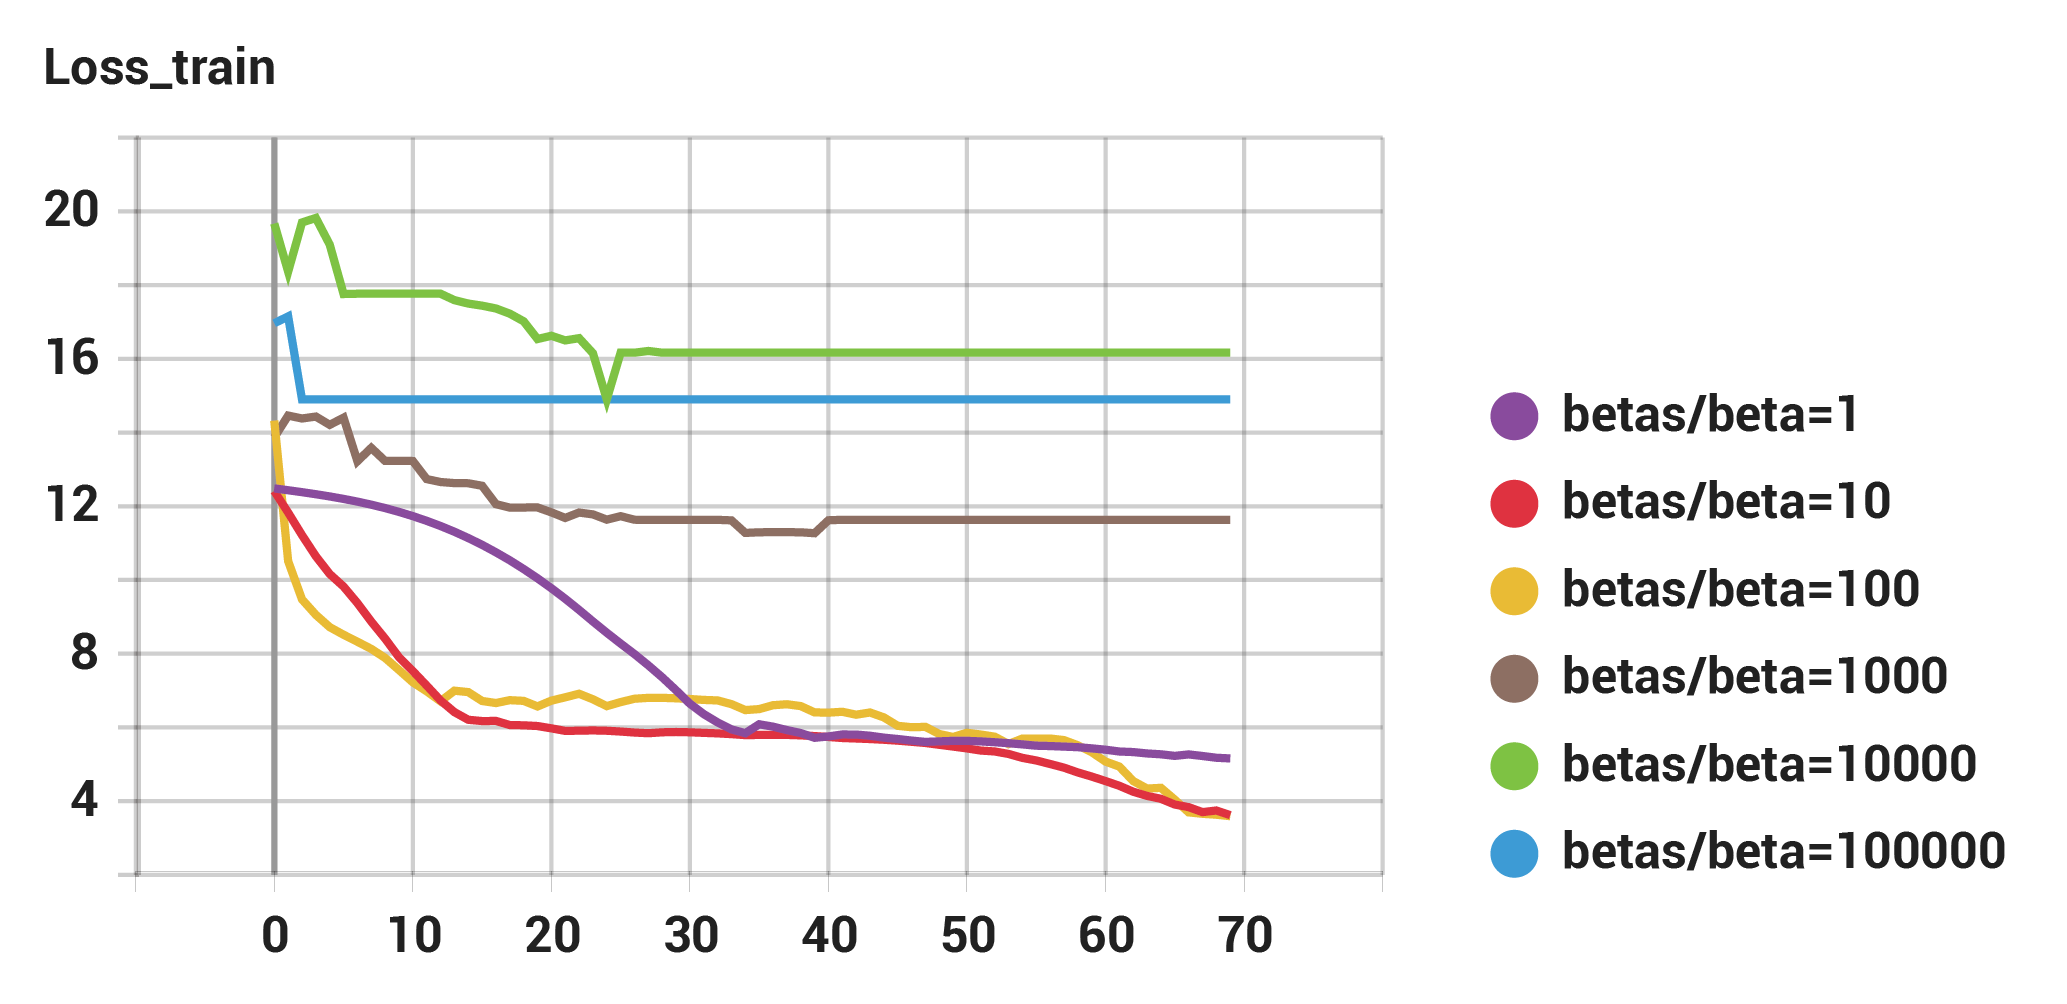
\includegraphics[width=0.9\textwidth]{figuras/betas_-Loss.png}   }
\caption{Training loss plot over the training epochs of a pointer network model for varying $\beta$ values. Training was done over only 10 data points in order o explore the ability of the model to overfit, the initial rational was that if a model cannot even overfit a minuscule dataset it is not suitable for training with the entire dataset or that it may even be be broken.}
\label{beta_loss}
\end{figure}